This chapter briefly reviews the concepts used throughout this work.


\section{Context-aware Systems}
Context-aware systems are those able to adapt their behavior according to changing circumstances without user intervention. Finkelstein and Savigni~\cite{finkelstein_framework_2001} describe a framework for context-aware services. Their approach is depicted in Figure~\ref{fig:finkelstein_framework}.

\begin{figure}[!htb]
  \centering
  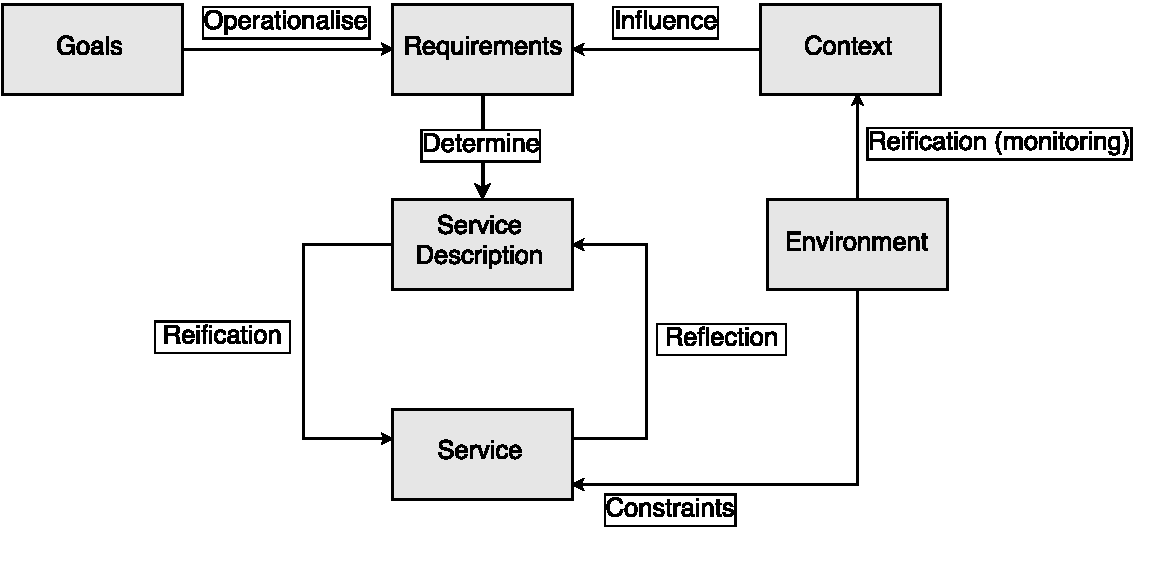
\includegraphics[width=.8\linewidth]{finkelstein_framework}
  \caption{Context-aware services framework by~\cite{finkelstein_framework_2001}}
\label{fig:finkelstein_framework}
\end{figure}

\emph{Environment} is whatever in the world provides a surrounding in which the agent is supposed to operate. The environment comprises such things as characteristics of the device that the agent is expected to operate in.
\emph{Context} is the reification of the environment. The \emph{context} provides a manageable, easily computer manipulable description of the \emph{environment}. A context-aware system should watch relevant environment properties and keep a runtime model that represents those properties. By reasoning about that model the system can change its behavior. A \emph{context} can be either an \emph{activator} of goals or a \emph{precondition} on the applicability of a certain strategy to reach a \emph{goal}.

A \emph{goal} is an objective the system should achieve. It is an abstract and long-term objective of the system. A \emph{requirement} operationalises a goal. It represents a more concrete and short-term objective that is directly achievable through actions performed by one or more agents. \emph{Service description} is the meta-level representation of the actual, real-world service. It should be a suitable formalism that allows services to be compared to requirements in order to identify runtime violations. Service provides the actual behavior as perceived by the user.

A \emph{reflective system} is a system which incorporates structures representing (aspects of) itself. A \emph{causal connection} between a model and a modeled element exists if one of them changes, this leads to a corresponding effect upon the other~\cite{maes_concepts_1987}. Following this approach, the system should keep a causal connection between the service and the description. The system adapts by manipulating the service description.
Following the requirements reflection vision~\cite{bencomo_requirements_2010}, a system should keep software requirements model at runtime, and use such model to drive the system adaptation.
